\section{VISIÓN COMPUTACIONAL}
    
    \subsection{PROCESAMIENTO DE IMÁGENES}
        Es la aplicación de operaciones del procesamiento de señales unidimensionales sobre imágenes, interpretadas como una señal bidimensional.
        
        \subsubsection{REPRESENTACIÓN DE IMÁGENES EN UNA COMPUTADORA}
        Una imagen $I$ está compuesta por píxeles $(x, y, v)$ cuyos componentes son una coordenada $(x, y) \in \mathbb{Z}^2$ y un valor $v \in \mathbb{Z}^c$, con $c$ el número de canales de color, siendo $c=1$ una imagen a escala de grises y $c=3$ una imagen a colores Rojo, Verde y Azúl (RGB por sus siglas en inglés), definida sobre un conjunto $\Omega$. 
        
        \begin{equation}
            \Omega = \{(x, y)| 1 \leq x \leq N_{columnas} \land 1 \leq y \leq N_{filas}\} \subset \mathbb{Z}^2
        \end{equation}
        
        la representación que se observa en la computadora se le llama modelo grid cell, donde cada píxel es un cuadrado pequeño o celda con una intensidad de grises o canales RGB \citep{10.5555/2584519} con valores $0 \leq I_{x, y} \leq 255$.
        
        Existen distintos tipos de imágenes con las que se suelte trabajar en el área de visión artificial, las más comunes son las ya citadas escalas de grises y RGB, sin embargo es común trabajar con imágenes binarias, es decir con valores 0 o 255, para la representación de máscaras o regiones de interés, al igual que espacios de color alternativos como HSV.

        \begin{figure}[H]
            \centering
            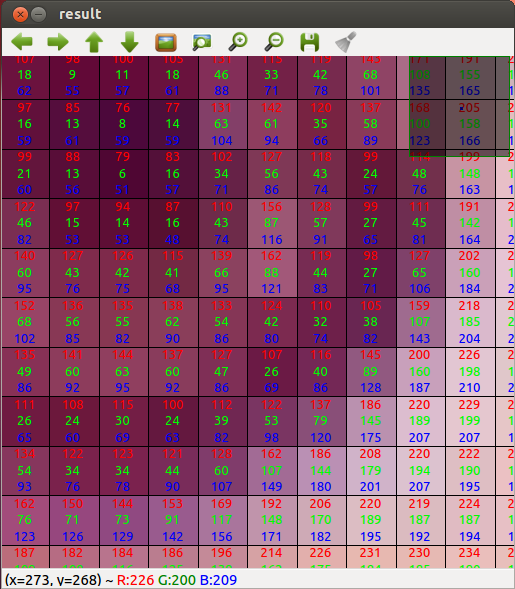
\includegraphics[scale=0.4]{imagenes/pixels}
            \caption[Intensidad de los canales de color RGB]{Intensidad de los canales de color RGB\\ Fuente: \citep{montabone_2012}}
        \end{figure}
		
        \subsubsection{CONVOLUCIÓN}
        Cuando se desea aplicar aplicar alguna transformación de alguna imagen $I$ a alguna imagen $I'$ como difuminados, realce de bordes o extracción de alguna característica, se debe aplicar un operador local lineal entre un filtro que acentúe la característica en la imagen $I$.
        
        El filtro denotado por $W$ es una matriz cuadrada de dimensión $(2k+1) \times (2k+1)$, aplicada en forma de ventana deslizante sobre cada pedazo de la misma dimensión de la imagen original, siendo $(x, y)$ el punto central de cada sección sobre la que se opera, se define la convolución como:
        
        \begin{equation}
            I'_{x,y} = \frac{1}{s} \sum_{i=-k}^{k} \sum_{j=-k}^{k} w_{i, j}\cdot I_{x+i, y+j}
        \end{equation}
        
        y se denota por el operador $*$ como $I' = I*W$ con $s$ un valor de escala \citep{10.5555/2584519}. Esta operación es equivalente a si se aplasta el filtro y la sección de la imagen en dos vectores, con el segundo vector al revés, y se realiza un producto punto o suma ponderada de sus valores.
        
        \begin{figure}[H]
        	\centering
        	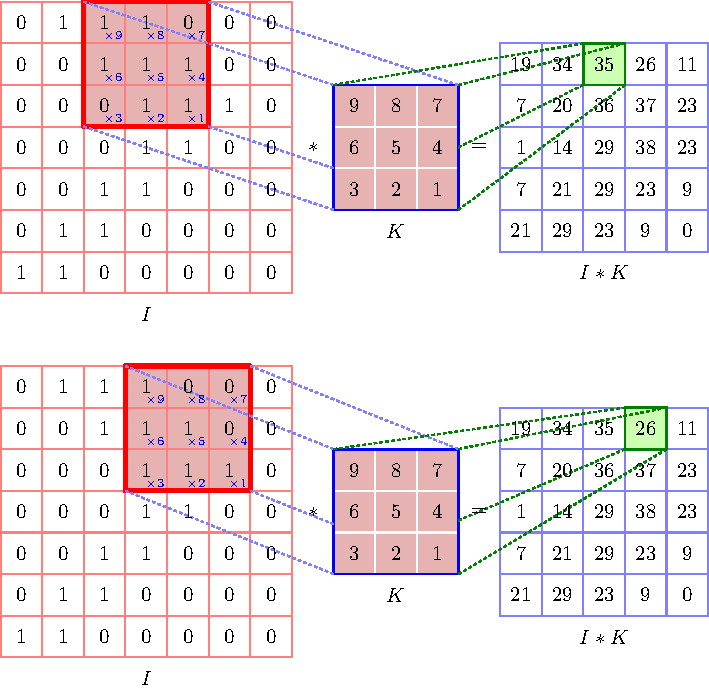
\includegraphics[scale=0.82]{imagenes/conv1}
        	\caption[Convolución del filtro $K$ con la imagen $I$]{convolución del filtro $K$ con la imagen $I$\\Fuente: elaboración propia}
        \end{figure}
    
    	\subsubsection{DETECCIÓN DE CONTORNOS}
    		
        
        \subsection{TRANSFORMACIONES MORFOLÓGICAS}
        	En tareas de imágenes binarias, el tipo más común de operaciones o filtros aplicados son las transformaciones morfológicas, llamadas así ya que modifican la estructura de los objetos binarios en la imagen, consisten en filtros llamados elementos estructurantes, los cuales son una matriz binaria que contiene un patrón bajo el cual se realiza una comparación o conteo píxel a píxel con recortes de la imagen, similar a una convolución 2D \citep{szeliski}
			\subsubsection{DILATACIÓN}
				Es la operación que consiste en dilatar los píxeles, cuenta cuántos píxeles en el recorte de la imagen que estén en la misma coordenada que los unos del elemento estructurante son distintos de cero, si existe por lo menos un píxel que cumple esta condición entonces el píxel central de la ventana deslizante se le asignará el valor distinto de cero especificado.
				
				Gráficamente se puede interpretar como engrosar los trazos de algún objeto binario incrementando píxeles en los bordes.
				
				\begin{figure}[H]
					\centering
					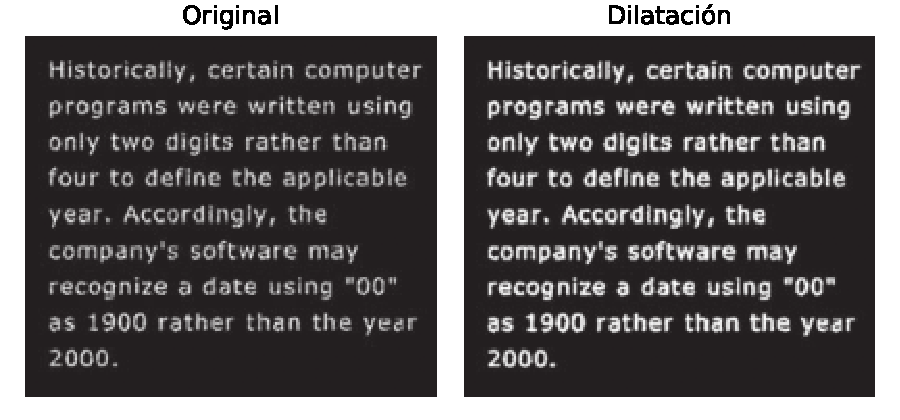
\includegraphics[scale=0.7]{imagenes/dilatacion}
					\caption[Dilatación sobre un conjunto de letras con discontinuidades]{dilatación sobre un conjunto de letras con discontinuidades\\Fuente: \citep{gonzalez}}
				\end{figure}	
						
			\subsubsection{EROSIÓN}
				Es la operación inversa a la dilatación, para esta operación, se realiza el mismo conteo de píxeles distintos de cero que encajen con la estructura del elemento estructurante, pero se asigna un valor positivo al centro solamente si el conteo es igual al número de elementos distintos de cero del filtro.
				
				\begin{figure}[H]
					\centering
					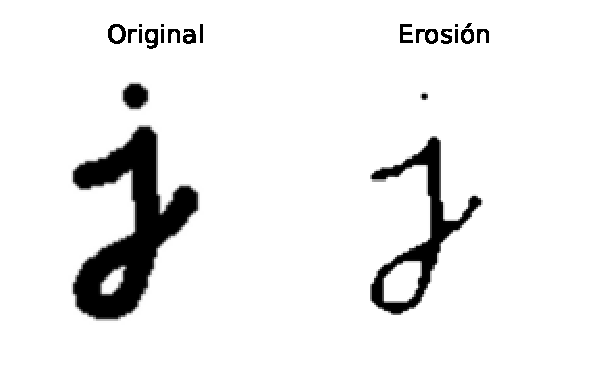
\includegraphics[scale=0.7]{imagenes/erosion}
					\caption[Erosión de una letra]{erosión de una letra\\Fuente: \citep{szeliski}}
				\end{figure}
				
				El resultado gráfico de esta operación es equivalente a reducir los bordes de los objetos haciéndolos más delgados o pequeños.
			\subsubsection{APERTURA}
				Es una operación que combina erosión seguido de dilatación en un solo paso, se usa para eliminar pequeños artefactos que no pertenecen a los objetos de interés que se buscan extraer, como ruido o falsas detecciones discontinuas.
				
				\begin{figure}[H]
					\centering
					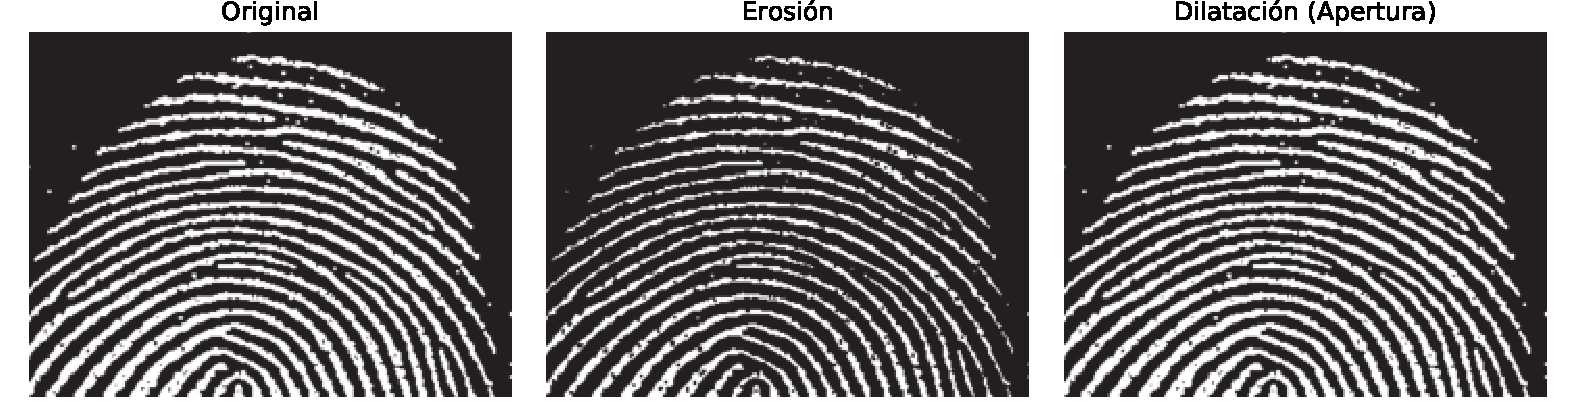
\includegraphics[scale=0.6]{imagenes/apertura}
					\caption[Apertura aplicada a una huella digital]{apertura aplicada a una huella digital para eliminar artefactos\\Fuente: \citep{gonzalez}}
				\end{figure}
				
				Al aplicar primero una erosión, se eliminan fragmentos discontinuos de menos píxeles que el tamaño de la ventana pero también se reduce el grosor de los objetos de interés, así que se aplica una dilatación, como los artefactos ya desaparecieron para ese momento, simplemente se restauran los objetos que pasaron la fase de erosión.
        \subsection{K-MEANS}
        	En español K-Medias, es un algoritmo nacido en el ámbito del procesamiento de señales y usado ampliamente en minería da datos para particionar un conjunto de $n$ observaciones en $k$ conglomerados o clusters, con el fin de clasificar a qué grupo pertenece cada observación o extraer información relevante de la relación entre los puntos de un mismo subconjunto.
        	
        	Debido a que se pretende que el algoritmo sea quien extraiga la información de los datos, la única entrada que se le provee es el número de clusters esperados, en base al cual se inicializan $k$ puntos aleatorios representando los centros de cada conglomerado. Al inicializarse aleatoriamente, se deben mejorar iterativamente las coordenadas de los centroides o medias denominados $\mu_i$.
        	
        	Se define una matriz binaria $R$ de dimensiones $m\times k$ dónde $m$ es el número de observaciones, esta matriz codifica en cada fila, representando a cada observación, el cluster al que pertenece, mediante un $1$ en la colúmna del cluster $i$ y $0$ en las demás. A cada elemento de $R$ se lo denominará como $r_{ij}$
        	
        	Se busca minimizar la distancia entre elementos de cada cluster, es decir la distancia de una observación con su respectivo centroide, esto se hace optimizando la función de costo:
        	
        	\begin{equation}
        		J = \sum_{i=1}^m\sum_{j=1}^k r_{ij}||x_i - \mu_j||^2
        	\end{equation}
        	
        	La minimización de $J$ se hace mediante dos etapas hasta convergencia. Primero la asignación de centroides a cada punto mediante la regla:
        	
        	\begin{equation}
        		r_{ij} = 
        		\begin{cases}
        			1 & si j = \underset{p}{argmin}||x_i - \mu_p||\\
        			0 & e.o.c
        		\end{cases}
        	\end{equation}
        
        	seguido del cómputo de nuevos centroides mediante el cálculo de la media de los puntos asignados al cluster $j$ en la anterior etapa \citep{bishop}.
        	
        	\begin{equation}
        		\mu_j = \frac{\sum_{i}r_{ij}x_i}{\sum_{i}r_{ij}}
        	\end{equation}
        
        	\begin{figure}[H]
        		\centering
        		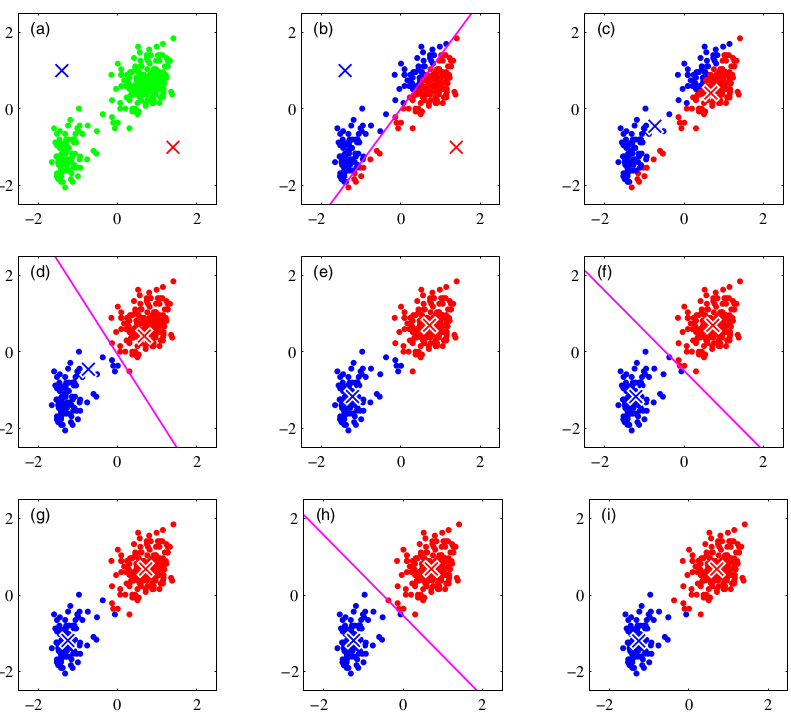
\includegraphics[scale=0.5]{imagenes/kmeans}
        		\caption[Ajuste iterativo de k-means]{ajuste iterativo de k-means\\Fuente: \citep{bishop}}
        	\end{figure}
        \subsection{FLOOD FILL}
        	Este algoritmo se usa cuando se desea rellenar un área delimitada por ciertos valores en una matriz, todas las herramientas de rellenado de color en programas de edición de imágenes usan una implementación.
        	
        	Consiste en recorrer recursivamente la matriz, marcando las posiciones ya visitadas hasta que ya no tenga a dónde ir, esta condición se cumple cuando todas las casillas de alrededor ya están marcadas como visitadas o de algún valor distinto al que se busca \citep{halim2013competitive}.\\
        	
        	{\setstretch{1.0}
        		\begin{algorithm}[H]
        			\caption{\textit{Flood Fill}}
        			\SetAlgoLined
        			\KwData{$mat:$ Matriz de valores}
        			\KwData{$y:$ coordenada vertical actual}
        			\KwData{$x:$ coordenada horizontal actual}
        			\KwData{$d:$ vector de direcciones}
        			\vspace{2mm}
        			\If{mat[$ y $][$x$] $\neq$ val}{
        				mat[$ y $][$x$] = marca \tcp*{se marca como visitado}
        				\For{i $\rightarrow$ \textbf{length} d}{
        					flood\_fill($mat$, $y$+d[$ i $].y, x+d[$ i $].x)
        				}
        			}
        			\tcc{si ya está visitado finaliza la rama de recursión}
        		\end{algorithm}
        	}
        	
%        \subsubsection{DIFUMINADO}
%        Para aplicar un difuminado o blur a una imagen se aplica comúnmente un filtro normal o gaussiano, para esto se define que el filtro se distribuye normal bivariante:
%        
%        \begin{equation}
%            W \sim \mathcal{N}\left(\mu=\begin{bmatrix}
%                                    0\\
%                                    0
%                                    \end{bmatrix},
%                                    \Sigma=
%                                    \begin{bmatrix}
%                                    \sigma^2 & 0\\
%                                    0 & \sigma^2
%                                    \end{bmatrix}\right)
%        \end{equation}
%        
%        Si generamos un filtro o kernel como una muestra de la distribución normal, de tamaño $6\sigma-1$ redondeado al entero impar más cercano, por la regla empírica de las tres desviaciones estándar, y escalado por $\frac{1}{s}$, obtenemos el un filtro que ponderará más los píxeles cercanos al centro, de manera que el difuminado mantendrá las características de cada sección de la imagen.
%        
%        \begin{figure}[H]
%            \centering
%            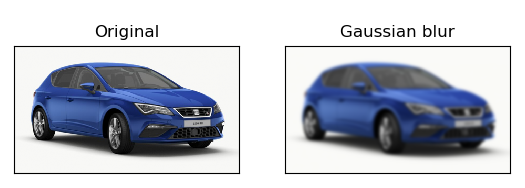
\includegraphics[scale=0.48]{imagenes/blur}
%            \caption{aplicación del filtro gaussiano\\ Fuente: Elaboración propia}
%        \end{figure}
%        % {\centering Fuente: Elaboración propia\par}
%        \subsubsection{DETECCIÓN DE BORDES}
%        Un borde es esencialmente un cambio brusco de intensidad de los valores de los píxeles en una sección de una imagen, de esta manera, para detectar bordes debemos aplicar algún tipo de suma ponderada que dé como resultado un valor alto si existe un cambio brusco de intensidad, y un valor bajo en caso contrario. 
%        Es bajo esta premisa que se propone el filtro Sobel \citep{sobel}, usado luego de aplicar un difuminado gaussiano, y consiste en una combinación entre una convolución gaussiana
%        $$\mathcal{G} = \begin{bmatrix}
%                                    1\\
%                                    2\\
%                                    1
%                        \end{bmatrix}$$
%        \noindent y una aproximación de la derivada parcial de la imagen en espacio discreto con $\Delta_x = \Delta_y = 1$ en cada dimensión
%        
%        $$\frac{\partial I_{x, y}}{\partial x} = \frac{I_{x+\Delta_x, y} - I_{x-\Delta_x, y}}{\Delta_x}$$
%        
%        $$\frac{\partial I_{x, y}}{\partial y} = \frac{I_{x, y+\Delta_y} - I_{x, y-\Delta_y}}{\Delta_y}$$
%        
%        \noindent dando como filtro unidimensional
%        
%        $$\mathcal{D} = \begin{bmatrix}
%                                    1 & 0 & -1
%                        \end{bmatrix}$$
%                        
%        \noindent combinando ambos filtros unidimensionales obtenemos el filtro Sobel para cada dimensión
%        \begin{equation}
%        \begin{aligned}
%        S_x &=  \begin{bmatrix}
%                 1\\
%                 2\\
%                 1
%                 \end{bmatrix}
%                 \begin{bmatrix}
%                 1 & 0 & -1
%                 \end{bmatrix}=
%                 \begin{bmatrix}
%                 1 &  0 &  -1\\
%                 2 &  0 &  -2\\
%                 1 &  0 &  -1\\
%                 \end{bmatrix}\\
%        S_y &=  \begin{bmatrix}
%                 1\\
%                 0\\
%                 -1
%                 \end{bmatrix}
%                 \begin{bmatrix}
%                 1 & 2 & 1
%                 \end{bmatrix}=
%                 \begin{bmatrix}
%                 1 &  2 &  1\\
%                 0 &  0 &  0\\
%                 -1 &  -2 &  -1\\
%                 \end{bmatrix}
%        \end{aligned}
%        \end{equation}
%        
%        \noindent al ser esta la derivada parcial con respecto de cada dirección, podemos calcular la magnitud mediante la norma $L_2$
%        
%        \begin{equation}
%            \nabla I_{x, y} = \sqrt{S_x^2 + S_y^2}
%        \end{equation}
%        
%        \noindent y la dirección del gradiente
%        
%        \begin{equation}
%            \theta = tan^{-1}\left(\frac{S_y}{S_x}\right)
%        \end{equation}
%        
%        \begin{figure}[H]
%            \centering
%            % 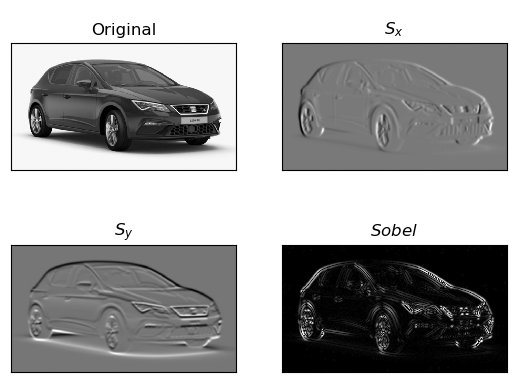
\includegraphics[scale=0.5]{imagenes/sobel_filters}
%            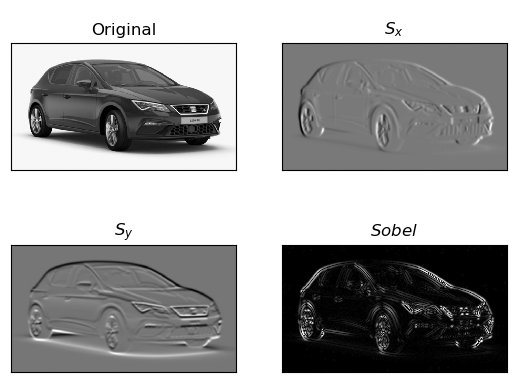
\includegraphics[scale=0.47]{imagenes/sobel_filters}
%            \caption{filtro Sobel por dimensiones y total\\ Fuente: Elaboración propia}
%        \end{figure}
%        % \vspace{-8mm}
%        % \begin{center}
%        %     Fuente: Elaboración propia
%        % \end{center}
%        \subsubsection{FILTRO CANNY}
%        Los bordes detectados por el filtro Sobel no son independientes de la resolución, por lo que pueden ser más gruesos o delgados dependiendo de la imagen, y detectar como bordes transiciones de iluminación que no lo son necesariamente, es con el fin de refinar este resultado que propone el filtro Canny, que se aplica a la salida de un filtro Sobel \citep{canny}.
%        Para aplicar este filtro primero se redondean las direcciones a múltiplos de $45^\circ$ y se procede a verificar si comparado con los píxeles vecinos en esa sección y esa orientación, es el valor máximo o no, en caso que no lo fuese se anula el valor del píxel volviéndolo $0$, caso contrario se continúa con el paso de probar límites de valores, dónde se eligen dos valores $t_{alto}$ y $t_{bajo}$, si un píxel cumple $I_{x,y} \ge t_{alto}$ entonces se considera borde, entonces se verifica cuáles de los 8 píxeles vecinos cumplen $I_{x\pm 1, y \pm 1} \ge t_{bajo}$, finalmente los píxeles que cumplan esta condición se marcan con el máximo valor de un píxel, $255$ y se repite el procedimiento. Si no se cumple la primera condición con el límite alto se asigna el valor $0$ al píxel, obteniendo así una imagen binaria donde los píxeles que representan un borde son de color blanco y los que no, son negros.
%        
%        \begin{figure}[H]
%            \centering
%            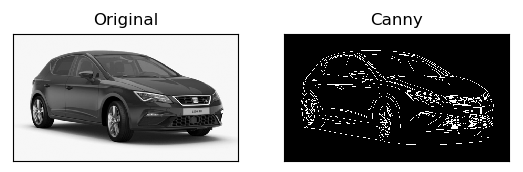
\includegraphics[scale=0.55]{imagenes/canny}
%            \caption{aplicación del filtro Canny\\ Fuente: Elaboración propia}
%        \end{figure}
